% use option [draft] for initial submission
%            [final] for the prepublication
\documentclass[qe,nameyear,draft]{econsocart}
%
%\usepackage{}
\RequirePackage[colorlinks,citecolor=blue,linkcolor=blue,urlcolor=blue,pagebackref]{hyperref}

\startlocaldefs

%%%%%%%%%%%%%%%%%%%%%%%%%%%%%%%%%%%%%%%%%%%%%%
%%                                          %%
%% Uncomment next line to change            %%
%% the type of equation numbering           %%
%%                                          %%
%%%%%%%%%%%%%%%%%%%%%%%%%%%%%%%%%%%%%%%%%%%%%%
%\numberwithin{equation}{section}
%%%%%%%%%%%%%%%%%%%%%%%%%%%%%%%%%%%%%%%%%%%%%%
%%                                          %%
%% For Assumption, Axiom, Claim, Corollary, %%
%% Lemma, Theorem, Proposition, Hypothezis, %%
%% Fact                                     %%
%% use \theoremstyle{plain}                 %%
%%                                          %%
%%%%%%%%%%%%%%%%%%%%%%%%%%%%%%%%%%%%%%%%%%%%%%
\theoremstyle{plain}
\newtheorem{axiom}{Axiom}
\newtheorem{theorem}{Theorem}
\newtheorem{claim}{Claim}
\newtheorem{lemma}[theorem]{Lemma}
\newtheorem*{fact}{Fact}
%%%%%%%%%%%%%%%%%%%%%%%%%%%%%%%%%%%%%%%%%%%%%%
%%                                          %%
%% For Definition, Example, Remark,         %%
%% Notation, Property                       %%
%% use \theoremstyle{remark}                %%
%%                                          %%
%%%%%%%%%%%%%%%%%%%%%%%%%%%%%%%%%%%%%%%%%%%%%%
\theoremstyle{remark}
\newtheorem{definition}{Definition}
\newtheorem*{example}{Example}
\newtheorem{remark}{Remark}

%%%%%%%%%%%%%%%%%%%%%%%%%%%%%%%%%%%%%%%%%%%%%%
%% Please put your definitions here:        %%
%%%%%%%%%%%%%%%%%%%%%%%%%%%%%%%%%%%%%%%%%%%%%%


\endlocaldefs

\begin{document}

\begin{frontmatter}

\title{A sample article title}
\runtitle{A sample running head title}

\begin{aug}
% use \particle for den|der|de|van|von (only lc!)
% [id=?,addressref=?,corref]{\fnms{}~\snm{}\ead[label=e?]{}\thanksref{}}
%
%% e-mail is mandatory for each author
%
%%% initials in fnms (if any) with spaces
%
\author[id=au1,addressref={add1,add11}]{\fnms{First}~\snm{Author}\ead[label=e1]{first@somewhere.com}}
\author[id=au2,addressref={add2}]{\fnms{Second}~\snm{Author}\ead[label=e2]{second@somewhere.com}}
\author[id=au3,addressref={add2}]{\fnms{Third}~\snm{Author}\ead[label=e3]{third@somewhere.com}}
%%%%%%%%%%%%%%%%%%%%%%%%%%%%%%%%%%%%%%%%%%%%%%
%% Addresses                                %%
%%%%%%%%%%%%%%%%%%%%%%%%%%%%%%%%%%%%%%%%%%%%%%
\address[id=add1]{%
\orgdiv{First Department of the First Author},
\orgname{University}}

\address[id=add11]{%
\orgdiv{Second Department of the First Author},
\orgname{University}}

\address[id=add2]{%
\orgdiv{Department of the Second and Third Authors},
\orgname{University}}
\end{aug}

%% Put support info here. Reminder: do not thank the handling coeditor anonymously or by name
\support{We thank four anonymous referees. The Editor should not be thanked anonymously or by name in this footnote, or elsewhere in the paper. The first author gratefully acknowledges
financial support from the National Science Foundation through Grant XXX-0000000.}
%
\coeditor{\fnm{[Name} \snm{Surname}; will be inserted later]}

\begin{abstract}
The abstract should summarize the contents of the paper. It should be clear,
descriptive, self-explanatory and not longer than 150 words. It should also be
suitable for publication in abstracting services. Please avoid using math formulas
as much as possible. We recommend 3--8 keywords and up to 3 JEL codes.
\end{abstract}


\begin{keyword}
\kwd{First keyword}
\kwd{second keyword}
\kwd{third keyword}
\end{keyword}

\begin{keyword}[class=JEL] %% alphabetical order
\kwd{First JEL}
\kwd{second JEL}
\end{keyword}

\end{frontmatter}
%%%%%%%%%%%%%%%%%%%%%%%%%%%%%%%%%%%%%%%%%%%%%%%%%%%%%%%%%%%%%%%%%%%%%%%%%
%%%% Main text entry area:
%%%%%%%%%%%%%%%%%%%%%%%%%%%%%%%%%%%%%%%%%%%%%%%%%%%%%%%%%%%%%%%%%%%%%%%%%

\section{Introduction}\label{s1}

This template helps you to create a properly formatted \LaTeXe\ manuscript.
Prepare your paper in the same style as used in this sample .pdf file.
Try to avoid excessive use of italics and bold face; underlining is generally banned (except for exceptional cases). Please do not use any \LaTeXe\ or \TeX\ commands that affect the layout or formatting of your document (i.e., commands like \verb|\textheight|, \verb|\textwidth|, etc.). Note that the Introduction should be Section~\ref{s1} it should not imediately follow the abstract without a heading.

\section{Section headings}
Here are some subsections:
\subsection{A subsection}
Regular text.
\subsubsection{A subsubsection}
Regular text.

\paragraph*{Paragraph heading} If you want to add mini-headings for paragraphs without numbers please use \verb|\paragraph*{}|.

\section{Text}

\subsection{Lists}

The following is an example of an \emph{itemized} list,
two levels deep.
\begin{itemize}
\item
This is the first item of an itemized list.  Each item
in the list is marked with a ``tick.''  The document
style determines what kind of tick mark is used.
\item
This is the second item of the list.  It contains another
list nested inside of it.
\begin{itemize}
\item This is the first item of an itemized list that
is nested within the itemized list.
\item This is the second item of the inner list.  \LaTeX\
allows you to nest lists deeper than you really should.
\end{itemize}
This is the rest of the second item of the outer list.
\item
This is the third item of the list.
\end{itemize}

The following is an example of an \emph{enumerated} list, two levels deep.
\begin{enumerate}[(ii)]
\item[(i)]
This is the first item of an enumerated list.  Each item
in the list is marked with a ``tick.''  The document
style determines what kind of tick mark is used.
\item[(ii)]
This is the second item of the list.  It contains another
list nested inside of it.
\begin{enumerate}
\item
This is the first item of an enumerated list that
is nested within.
\item
This is the second item of the inner list.  \LaTeX\
allows you to nest lists deeper than you really should.
\end{enumerate}
This is the rest of the second item of the outer list.
\item [(iii)]
This is the third item of the list.
\end{enumerate}

Do not use (1), (2), etc.\ for items in order to avoid confusion with numbered equations.

\subsection{Punctuation}
Avoid unnecessary hyphenation; many hyphenated words can be treated as one or two words.
Dashes come in three sizes: a hyphen, an intra-word dash like ``$U$-statistics'' or ``the time-homogeneous model'';
a medium dash (also called an ``en-dash'') for number ranges or between two equal entities like ``1--2'' or ``Cauchy--Schwarz inequality'';
and a punctuation dash (also called an ``em-dash'') in place of a comma, semicolon,
colon or parentheses---like this.

Generating an ellipsis \ldots\ with the right spacing
around the periods requires using \verb|\ldots|.

\textit{Theoretical Economics} is using longer spaces after periods, please add \verb|\| after periods that are not at the end of a sentence, in order to have regular spaces. For example, if there is an abbreviation (e.g., econ. theory) which is not the end of an article but appears in a middle of a sentence, please code it as \verb|(e.g., econ.\ theory)|. 

\subsection{Citation}
Only include in the reference list entries for which there are text citations,
and make sure all citations are included in the reference list.
Simple author and year cite: \citet{b1}. 
Multiple bibliography items cite: \citet{b2,b3,b4,b5}.
Author only cite: \citeauthor{b4}.
Year only cite: (\citeyear{b4}). Citing bibliography with object \citet[Theorem 1]{b1}. Citing within brackets is done with the same commands (e.g., \citet{b2,b3,b4}).

\section{Fonts}
Please use text fonts in text mode, e.g.:
\begin{itemize}
\item[]\textrm{Roman} \verb|\textrm{}|
\item[]\textit{Italic} \verb|\textit{}|
\item[]\textbf{Bold} \verb|\textbf{}|
\item[]\textsc{Small Caps} \verb|\textsc{}|
\item[]\textsf{Sans serif} \verb|\textsf{}|
\item[]\texttt{Typewriter} \verb|\texttt{}|
\end{itemize}
Please use mathematical fonts in mathematical mode, e.g.:
\begin{itemize}
\item[] $\mathrm{ABCabc123}$ \verb|\mathrm{}|
\item[] $\mathit{ABCabc123}$ \verb|\mathit{}|
\item[] $\mathbf{ABCabc123}$ \verb|\mathbf{}|
\item[] $\boldsymbol{ABCabc123\alpha\beta\gamma}$ \verb|\boldsymbol{}|
\item[] $\mathcal{ABC}$ \verb|\mathcal{}|
\item[] $\mathbb{ABC}$ \verb|\mathbb{}|
\item[] $\mathsf{ABCabc123}$ \verb|\mathsf{}| 
\item[] $\mathtt{ABCabc123}$ \verb|\mathtt{}|
\item[] $\mathfrak{ABCabc123}$ \verb|\mathfrak{}|
\end{itemize}
Note that \verb|\mathcal, \mathbb| belongs to capital letters-only font typefaces.

\section{Notes}
Footnotes\footnote{This is an example of a footnote.}
pose no problems in text.\footnote{Note that footnote number is after punctuation.} Please do not add footnotes on math. 

\section{Numbers}
A decimal point always should be preceded by a whole number and never should be left ``naked.'' Decimal expressions of numbers less than 1 always should be preceded by a zero (0) to enhance the visibility of the decimal. For example, .3 should be 0.3.   This applies to text, tables, and figures.


\section{Quotations}

Text is displayed by indenting it from the left margin. There are short quotations
\begin{quote}
This is a short quotation.  It consists of a
single paragraph of text.  There is no paragraph
indentation. It should be coded between \verb|\begin{quote}| and \verb|\end{quote}|.
\end{quote}
and longer ones.
\begin{quotation}
This is a longer quotation.  It consists of two paragraphs
of text.  The beginning of each paragraph is indicated
by an extra indentation.

This is the second paragraph of the quotation.  It is just
as dull as the first paragraph. It should be coded between \verb|\begin{quotation}| and \verb|\end{quotation}|.
\end{quotation}

\section{Environments}

Please use regular counters (Theorem 1) as opposed to counters belonging on sections (Theorem 3.1). Results (Lemmas, Propositions, Theorems, Claims) can be on the same or different counters.

\subsection{Examples for \emph{\texttt{plain}}-style environments}

\begin{theorem}\label{th1}
This is the body of Theorem \ref{th1}.
\end{theorem}


\begin{proof}
This is the body of the proof of the theorem above.
\end{proof}

\begin{claim}\label{cl1}
This is the body of Claim \ref{cl1}. 
\end{claim}



\begin{axiom}\label{ax1}
This is the body of Axiom \ref{ax1}. Axioms should be on a different counter from results (e.g. Theorems, Propositions, Lemmas).
\end{axiom}

\begin{theorem}[Title of the Theorem]\label{th2}
This is the body of Theorem \ref{th2}. Theorem~\ref{th2} has additional title.
\end{theorem}

\begin{lemma}\label{le1}
This is the body of Lemma \ref{le1}. Lemma \ref{le1} is numbered after
Theorem \ref{th2} because we used \verb|[theorem]| in \verb|\newtheorem|.
\end{lemma}

\begin{fact}
This is the body of the fact. Fact is unnumbered because we used the command \verb|\newtheorem*|
instead of \verb|\newtheorem|.
\end{fact}

\begin{proof}[Proof of Theorem \ref{th2}]
This is the body of the proof of Theorem \ref{th2}.
\end{proof}


\subsection{Examples for \emph{\texttt{remark}}-style environments}

The following environments can be numbered or not; if numbered, they should be on different counters from results.

\begin{definition}\label{de1}
This is the body of Definition \ref{de1}. Definitions should be on a different counter from results (e.g. Theorems, Propositions, Lemmas).
\end{definition}

\begin{example}
This is the body of the example. Example is unnumbered because we used \verb|\newtheorem*|
instead of \verb|\newtheorem|.
\end{example}

\begin{remark}
This is the body of the remark. 
\end{remark}

\section{Equations and the like}
Only number equations to which there is a subsequent reference.
See equations below (\ref{ccs})--(\ref{e7}). Please punctuate equations as you would punctuate a sentence, that is add a comma between two equations and add a period if it ends a sentence.

Two equations:
\begin{equation}
    C_{s}  =  K_{M} \frac{\mu/\mu_{x}}{1-\mu/\mu_{x}} \label{ccs}
\end{equation}
and
\begin{equation}
    G = \frac{P_{\mathrm{opt}} - P_{\mathrm{ref}}}{P_{\mathrm{ref}}}  100(\%).
\end{equation}
Equation arrays:
\begin{eqnarray}
  \frac{dS}{dt} & = & - \sigma X + s_{F} F,\\
  \frac{dX}{dt} & = &   \mu    X,\\
  \frac{dP}{dt} & = &   \pi    X - k_{h} P,\\
  \frac{dV}{dt} & = &   F.
\end{eqnarray}
One long equation, note that the equation number is on the last line:
\begin{eqnarray}
 \mu_{\text{normal}} & = & \mu_{x} \frac{C_{s}}{K_{x}C_{x}+C_{s}}  \nonumber\\
                     & = & \mu_{\text{normal}} - Y_{x/s}\bigl(1-H(C_{s})\bigr)(m_{s}+\pi /Y_{p/s})\nonumber\\
                     & = & \mu_{\text{normal}}/Y_{x/s}+ H(C_{s}) (m_{s}+ \pi /Y_{p/s}).\label{e7}
\end{eqnarray}
Note that variables made of more than one letter should use command \verb|\mathit|,
e.g., $\mathit{sov}=550$, where $\mathit{sov}$ is sum of votes. Abbreviations used in subscripts or superscripts should use \verb|\mathrm|,
e.g., $t_{\mathrm{max}}-t_{\mathrm{min}} =10$. Operator names should use \verb|\operatorname|, e.g. $\operatorname{AR}(1)$. Also, note that $\emptyset$ symbol is preferred to $\varnothing$.

\section{Tables and figures}
Cross-references to labeled tables: As you can see in Table~\ref{sphericcase}
and also in Table~\ref{parset}.

Sample of cross-reference to figure: Figure~\ref{penG} shows that it is not easy to get something on paper. Note that figures will be in grayscale in the printed version.

\begin{table*}
\caption{The spherical case ($I_1=0$, $I_2=0$).}
\label{sphericcase}
\begin{tabular}{@{}lrrrrc@{}@{}}
\hline
Equil. Points
& \multicolumn{1}{c}{$x$}
& \multicolumn{1}{c}{$y$}
& \multicolumn{1}{c}{$z$}
& \multicolumn{1}{c}{$C$}
& S \\
\hline
$L_1$    & $-$2.485252241 & 0.000000000    & 0.017100631    & 8.230711648    & U \\
$L_2$    & 0.000000000    & 0.000000000    & 3.068883732    & 0.000000000    & S \\
$L_3$    & 0.009869059    & 0.000000000    & 4.756386544    & $-$0.000057922 & U \\
$L_4$    & 0.210589855    & 0.000000000    & $-$0.007021459 & 9.440510897    & U \\
$L_5$    & 0.455926604    & 0.000000000    & $-$0.212446624 & 7.586126667    & U \\
$L_6$    & 0.667031314    & 0.000000000    & 0.529879957    & 3.497660052    & U \\
$L_7$    & 2.164386674    & 0.000000000    & $-$0.169308438 & 6.866562449    & U \\
$L_8$    & 0.560414471    & 0.421735658    & $-$0.093667445 & 9.241525367    & U \\
$L_9$    & 0.560414471    & $-$0.421735658 & $-$0.093667445 & 9.241525367    & U \\
$L_{10}$ & 1.472523232    & 1.393484549    & $-$0.083801333 & 6.733436505    & U \\
$L_{11}$ & 1.472523232    & $-$1.393484549 & $-$0.083801333 & 6.733436505    & U \\
\hline
\end{tabular}
\legend{This is how table note should be presented.
Please do not use asterisks or bold face to denote statistical significance.
We encourage authors to report standard errors and coverage sets or confidence intervals.}

\end{table*}

\begin{table}
\caption{Sample posterior estimates for each model.}
\label{parset}
%
\begin{tabular}{@{}lcrcrrr@{}@{}}
\hline
& & & &\multicolumn{3}{c}{Quantile} \\
\cline{5-7}
Model
& Parameter
& \multicolumn{1}{c}{Mean}
& Std. Dev.
& \multicolumn{1}{c}{2.5\%}
& \multicolumn{1}{c}{50\%}
& \multicolumn{1}{c@{}}{97.5\%} \\
\hline
{Model 0} & $\beta_0$ & $-$12.29 & 2.29 & $-$18.04 & $-$11.99 & $-$8.56 \\
          & $\beta_1$ & 0.10     & 0.07 & $-$0.05  & 0.10     & 0.26    \\
          & $\beta_2$ & 0.01     & 0.09 & $-$0.22  & 0.02     & 0.16    \\[6pt]
{Model 1} & $\beta_0$ & $-$4.58  & 3.04 & $-$11.00 & $-$4.44  & 1.06    \\
          & $\beta_1$ & 0.79     & 0.21 & 0.38     & 0.78     & 1.20    \\
          & $\beta_2$ & $-$0.28  & 0.10 & $-$0.48  & $-$0.28  & $-$0.07 \\[6pt]
{Model 2} & $\beta_0$ & $-$11.85 & 2.24 & $-$17.34 & $-$11.60 & $-$7.85 \\
          & $\beta_1$ & 0.73     & 0.21 & 0.32     & 0.73     & 1.16    \\
          & $\beta_2$ & $-$0.60  & 0.14 & $-$0.88  & $-$0.60  & $-$0.34 \\
          & $\beta_3$ & 0.22     & 0.17 & $-$0.10  & 0.22     & 0.55    \\
\hline
\end{tabular}
%
\end{table}

\begin{figure}
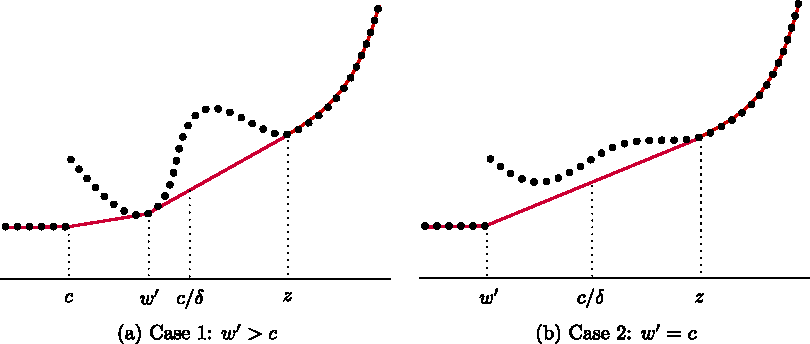
\includegraphics{figure_sample}
\caption{The dotted lines show the values of $u(x)$ for $x$ in the discrete support of $F$. The solid lines show $u_\textrm{conv}(x)$.}
\label{penG}
\end{figure}


%%%%%%%%%%%%%%%%%%%%%%%%%%%%%%%%%%%%%%%%%%%%%%
%% Example with single Appendix:            %%
%%%%%%%%%%%%%%%%%%%%%%%%%%%%%%%%%%%%%%%%%%%%%%
\begin{appendix}
\section*{Title}\label{appn} %% if no title is needed, leave empty \section*{}.
Appendices should be provided in \verb|{appendix}| environment. If there is only one appendix,
then please refer to it in text as \ldots\ in the \hyperref[appn]{Appendix}.
\end{appendix}

%%%%%%%%%%%%%%%%%%%%%%%%%%%%%%%%%%%%%%%%%%%%%%
%% Example with multiple Appendixes:        %%
%%%%%%%%%%%%%%%%%%%%%%%%%%%%%%%%%%%%%%%%%%%%%%
\begin{appendix}
\section{Title of the first appendix}\label{appA}
If there are more than one appendix, then please refer to it
as \ldots\ in Appendix \ref{appA}, Appendix \ref{appB}, etc.

\section{Title of the second appendix}\label{appB}
\subsection{First subsection of Appendix \protect\ref{appB}}\label{appB1}

If your appendix is long, make sure to divide it into subsections and refer to them in text. Use the standard \LaTeX\ commands for headings in \verb|{appendix}|.
Headings and other objects will be numbered automatically.
\begin{equation}
\mathcal{P}=(j_{k,1},j_{k,2},\dots,j_{k,m(k)}). \label{path}
\end{equation}

Sample of cross-reference to formula (\ref{path}) in Appendix \ref{appB1}.
Note that it is better to refer to Appendix \ref{appB1} as opposed to Appendix \ref{appB}, because it is easier for the reader to locate the necessary place. \end{appendix}

%%%%%%%%%%%%%%%%%%%%%%%%%%%%%%%%%%%%%%%%%%%%%%
%% Bibliography:                            %%
%%%%%%%%%%%%%%%%%%%%%%%%%%%%%%%%%%%%%%%%%%%%%%
%% IMPORTANT: References in the bibliography should be complete, 
%% including the first and last names, and date of publication.

%% If your bibliography is in bibtex format, uncomment commands:
%\bibliographystyle{qe} % Style BST file
%\bibliography{bibliography}  % Bibliography file (usually '*.bib')

%% Or include bibliography directly:

\begin{thebibliography}{}
%
\bibitem[\protect\citeauthoryear{Aumann}{1987}]{b1}
Aumann, Robert (1987),
``Correlated equilibrium as an expression of Bayesian rationality.''
\textit{Econometrica}, 55 (1), 1--18.
\endbibitem

\bibitem[\protect\citeauthoryear{Peck}{1994}]{b2}
Peck, James (1994),
``Competition in transactions mechanisms: The emergence of competition.''
Unpublished Manuscript, Ohio State University.
\endbibitem

\bibitem[\protect\citeauthoryear{Enelow and Hinich}{1990}]{b3}
Enelow, James, and Melvin Hinich, eds. (1990),
\textit{Advances in the Spatial Theory of Voting}.
Cambridge University Press, Cambridge, U.K.
\endbibitem

\bibitem[\protect\citeauthoryear{Wittman}{1990}]{b4}
Wittman, Donald (1990),
``Spatial strategies when candidates have policy preferences.''
In \textit{Advances in the Spatial Theory of Voting}
(M. Hinich and J. Enelow, eds.), 66--98,
Cambridge University Press, Cambridge, U.K.
\endbibitem

\bibitem[\protect\citeauthoryear{Cahuc, Postel-Vinay and Robin}{2006}]{b5}
Cahuc, P., F. Postel-Vinay, and J.-M. Robin (2006), 
``Supplement to `Wage bargaining with on-the-job search: Theory and evidence'.''
\textit{Quantitative Economics Supplemental Material}.
\endbibitem
\end{thebibliography}

\end{document}
